\vspace{40px} \section{Modulated signal spectrum}
The spectrum analysis is helpful for a better understanding of the behavior of the BPSK modulation technique. Analyzing the spectrum provides insights into the distribution of signal power across different frequencies. In this section, there will be the analysis an the plots of a periodic \texttt{1010} sequence and a randomly generated sequence.



\subsection{Periodic \texttt{1010} sequence signal}
To analyze and plot the spectrum of a periodic \texttt{1010} sequence signal some important values should be calculated. The $\omega_0$ value, which is the angular carrier frequency, the value, representing the base harmonic frequency and $k$, which is the range in which the spectrum will be calculated. The first two values may be calculated with the following expression:

\begin{equation*}
    \omega_0 = 2\pi f_0 \hspace{30px} \Omega = \frac{\pi}{\tau}
\end{equation*}

\noindent The $k$ range is a range of $n$ indexes around the carrier frequency central index, $k_0 = \omega_0 / \Omega$. These values can be easily obtained by running the below-displayed code snippet.

\begin{lstlisting}
    % anguolar carrier frequency
    omega_0 = 2 * pi * f0; 

    % base harmonic angoular frequency 
    OMEGA = pi / tau; 

    % Carrier frequency central index
    k_0 = omega_0 / OMEGA;

    % Define range of indexes for spectrum
    K = k_0 + (-10 : 10);
\end{lstlisting}

\noindent At this point, the BPSK spectrum can be calculated. To do so it is necessary to calculate the Fourier series coefficient for the BASK\footnote{Which stands for Binary Amplitude Shift Keying} modulation type using the following equation:

\begin{equation*}
    C_{BASK}(k) = j\frac{U}{4} \frac{\sin\left[ \left( k\Omega - \omega_0 \right) \frac{\tau}{2}\right]}{\left( k\Omega - \omega_0 \right) \frac{\tau}{2}}
\end{equation*}

\noindent Now that the BASK coefficients are calculated, the BPSK coefficients are easy to be computed:

\begin{equation*}
    C_{BPSK}(k) = C_{BASK}(k) \left[ e^{+jk\Omega\frac{\tau}{2}} - e^{-jk\Omega\frac{\tau}{2}} \right]
\end{equation*}

\noindent These two complex equations can be computed in MATLAB with the help of the \texttt{sinc} function as follows:

\begin{lstlisting}
    % Phase value of the spectral function
    phase = (K * OMEGA - omega_0) * tau / 2;

    C_BASK = sinc(phase / pi) * U / 4 * 1j; % fourirer series coefficient, BASK

    % BPSK spectrum for periodocal '1' and '0' sequence (...1 0 1 0 1 0 1 0 1 0...)
    C_BPSK = C_BASK .* ( exp(1j * K * OMEGA * tau / 2) -  exp(- 1j * K * OMEGA * tau / 2));
\end{lstlisting}

\noindent After numerically calculating the spectrum, it is very important to plot the result by running the following code snippet.

\begin{lstlisting}
    % creates figure and settings
    f = figure(2);
    f.Name = 'Analysis of BPSK spectrum';
    f.NumberTitle = 'off';
    f.Position = [200, 120, 1200, 600];
    
    % plot 1st result
    stem( K * OMEGA / (2 * pi), abs(C_BPSK), 'b' ), grid on,
    xlabel('Frequency [GHz]'), ylabel('Amplitude, [V]'), title('Amplitude Spectrum of periodic signal')
    ylim([-0.05, 0.35]);
\end{lstlisting}

\noindent By observing the plot displayed in figure\,\ref{fig:periodic-signal-spectrum} it is noticeable that the carrier component in the center of the plot is zero: this is the quirk of the BPSK modulation. Sure enough, the two BASK components subtract at the center of the spectrum but add up in the other cases due to the opposite phase of the formula. 

\begin{figure}[h]
    \centering
    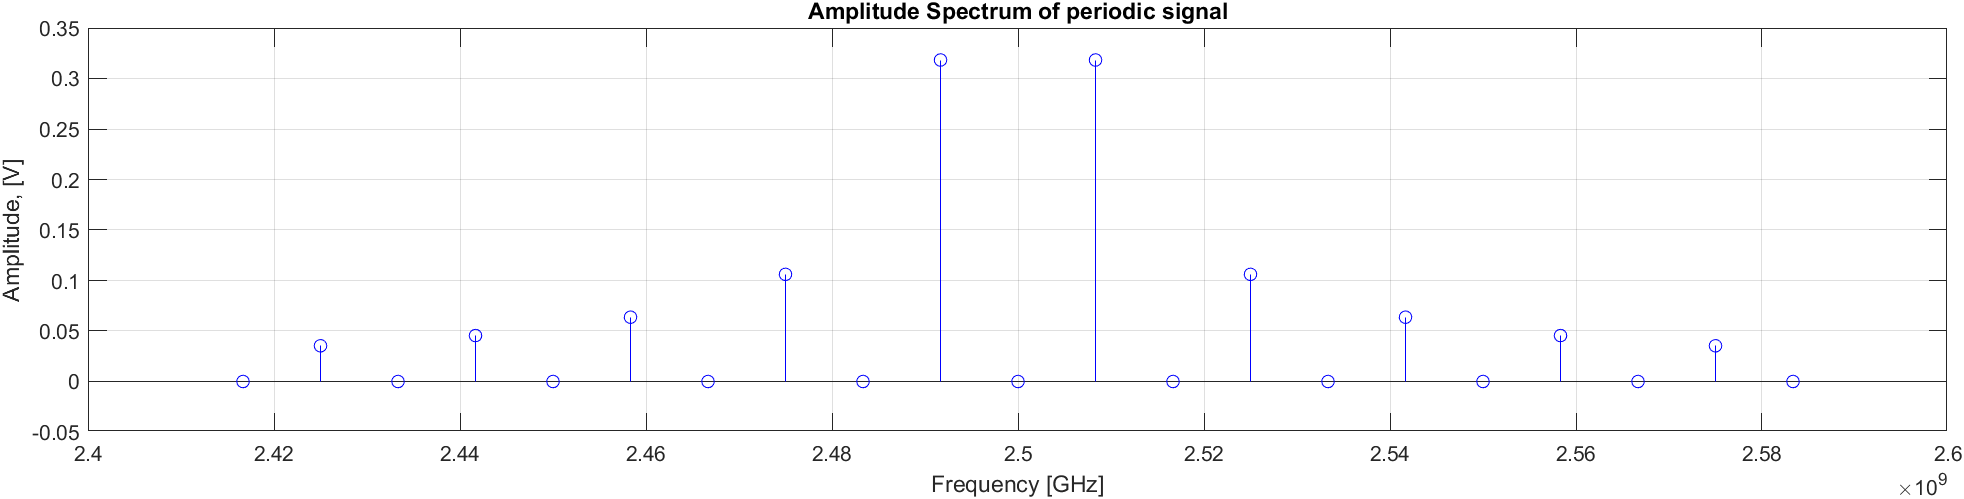
\includegraphics[width = \textwidth]{../res/imgs/periodic-signal-spectrum.png}
    \caption{BPSK periodic signal spectrum.}
    \label{fig:periodic-signal-spectrum}
\end{figure}


\subsection{Random sequence signal}
After plotting and analyzing the spectrum in the case of a periodic signal, it would be important to analyze the spectrum of a random signal as well. To do so it is necessary to get the power spectral density of the BPSK signal, which is double the power spectral density of the BASK modulation:

\begin{equation*}
    G_{BASK}(\omega) = 2\tau|C_{BASK}(\omega)|^2
\end{equation*}

\noindent Consequently the power spectral density of the BPSK signal, called $G_{BPSK}$, can be computed using the following MATLAB script.

\begin{lstlisting}
    % Power Spectral Density (PSD) for random input signal
    omega = ( K(1) : 1/100 : K(end) ) * OMEGA; % angoular frequency 

    phase = (omega - omega_0 ) * tau / 2; % continuous phase 
    S_BASK =  2 * tau * sinc(phase / pi ) * U / 4 * 1j;

    % PSD as a normalized squarred spectral function
    G_BPSK = 1/ tau * abs(S_BASK) .^2;
\end{lstlisting}

\noindent Eventually, as for the spectrum of a periodic signal, the graph can be plotted and generated using the following script.

\begin{lstlisting}
    % creates figure and settings
    f = figure(3);
    f.Name = 'Analysis of BPSK spectrum';
    f.NumberTitle = 'off';
    f.Position = [200, 120, 1200, 600];

    % plot 2nd result
    plot( omega / (2 * pi), G_BPSK, 'b' ), grid on,
    xlabel('Frequency [GHz]'), ylabel('PSD'), title('PSD of random signal')
    ylim([-0.1e-8, 1.6e-8]);
\end{lstlisting}

\noindent The result is that the spectrum of the BPSK signal is extremely high if compared with the BASK and BFSK spectrum due to its particular properties (figure\,\ref{fig:random-signal-spectrum}): the phase shift of $\pi$ doubles the PSD in comparison with the BASK and the BFSK making this modulation technique the most efficient one out of the three.

\begin{figure}[h]
    \centering
    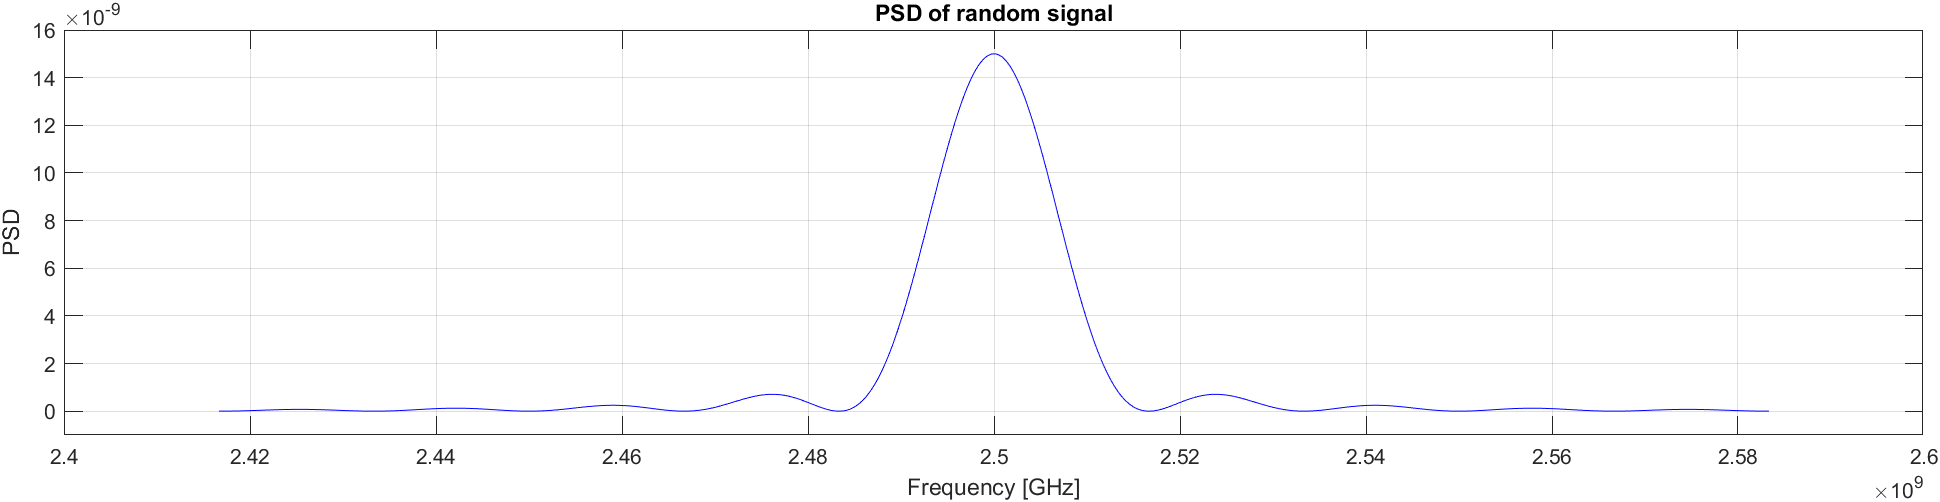
\includegraphics[width = \textwidth]{../res/imgs/random-signal-spectrum.png}
    \caption{BPSK random signal spectrum.}
    \label{fig:random-signal-spectrum}
\end{figure}